\documentclass{article}
\usepackage{tikz}
\usetikzlibrary{arrows}

% type, redundancy, required, lambda 
\newcommand{\modelgraphlabel}[4]{$#1$ \\ $r=#2$ \\ $q=#3$ \\ $\lambda=#4$}
\newcommand{\scale}{8}

\begin{document}

% 125 State (3 Components)
% draw - outline, fill - color!alpha, align - allows for manual linebreak
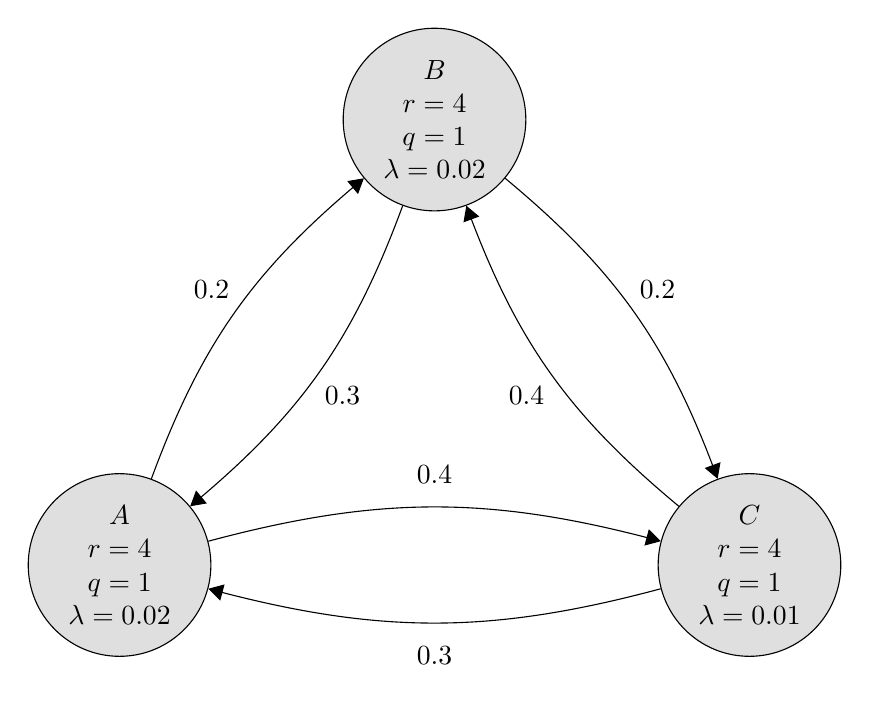
\begin{tikzpicture}[scale = 1, auto = left, every node/.style = {circle, draw = black, fill = gray!25}, bend angle = 90]
	\node (A) at (0, 0) [align = center] {\modelgraphlabel{A}{4}{1}{0.02}};
	\node (B) at (\scale / 2, \scale / 2^0.5) [align = center] {\modelgraphlabel{B}{4}{1}{0.02}};
	\node (C) at (\scale, 0) [align = center] {\modelgraphlabel{C}{4}{1}{0.01}};

  	\foreach \from/\phiEdge/\to in {A/0.2/B, A/0.4/C, B/0.3/A, B/0.2/C, C/0.3/A, C/0.4/B}
    	\path (\from) edge [-triangle 60, bend left=15] node[fill=none, draw=none] {\phiEdge} (\to);
\end{tikzpicture} 

\end{document}